
\documentclass[11pt,a4paper]{article}
\usepackage[utf8]{inputenc}
\usepackage[T1]{fontenc}
\usepackage[french]{babel}
\usepackage{lmodern}
\usepackage{geometry}
\usepackage{xcolor}
\usepackage{graphicx}
\usepackage{booktabs}
\usepackage{longtable}
\usepackage{array}
\usepackage{amsmath}
\usepackage{hyperref}
\usepackage{listings}
\geometry{margin=2.1cm}
\hypersetup{colorlinks=true, linkcolor=blue, urlcolor=blue}
\definecolor{codebg}{RGB}{245,246,248}
\lstset{
  basicstyle=\ttfamily\small,
  backgroundcolor=\color{codebg},
  frame=single,
  breaklines=true,
  columns=fullflexible
}
\title{\textbf{Guide complet du workflow}\\Projet de stéganographie LSB et détection}
\author{Projet de traitement d'images}
\date{12 juin 2026}
\begin{document}
\maketitle
\tableofcontents
\newpage

\section{But du projet}
Ce projet montre une chaîne complète de traitement d'images autour de la stéganographie LSB. Il ne s'agit pas seulement de donner un verdict automatique. Le but est de rendre visibles les transformations : image RGB, canaux rouge/vert/bleu, plans de bits, différence amplifiée, caractéristiques statistiques, puis classification.

L'application permet trois services :
\begin{itemize}
  \item \textbf{Détecter} si une image ressemble à une image contenant un message LSB.
  \item \textbf{Cacher du texte} dans une image en modifiant les bits de poids faible.
  \item \textbf{Extraire du texte} depuis un PNG produit par notre application.
\end{itemize}

\subsection*{Question centrale à savoir expliquer}
La question du projet est : comment une modification presque invisible dans une image peut-elle devenir mesurable ? La réponse est que l'oeil humain regarde surtout les structures visibles, alors que le traitement d'images peut isoler les couches numériques faibles, comme les LSB, et mesurer leurs distributions.

Il faut donc présenter le projet comme une chaîne logique :
\begin{center}
\texttt{pixels -> bits -> plans LSB -> features -> modèles -> verdict}
\end{center}

\section{Architecture logique du système}
Le projet est divisé en quatre blocs. Cette séparation est importante parce qu'elle permet d'expliquer clairement ce que fait chaque partie.

\begin{longtable}{p{3.4cm}p{5.2cm}p{5.2cm}}
\toprule
Bloc & Comment il fonctionne & Pourquoi il existe \\
\midrule
Insertion & Convertit un message texte en bits et remplace les LSB des valeurs RGB. & Créer des exemples stego contrôlés et montrer concrètement la stéganographie. \\
Extraction & Relit les LSB, reconstruit les octets, puis décode le texte UTF-8. & Prouver que le message est vraiment dans l'image, pas seulement que l'image est classée stego. \\
Extraction de features & Transforme une image en nombres : LSB, textures, histogrammes et moments. & Un modèle ne comprend pas une image comme un humain ; il a besoin de mesures numériques. \\
Classification & Compare les features à ce qui a été appris sur clean/stego. & Donner une décision automatique et quantifiée. \\
\bottomrule
\end{longtable}

Ce découpage aide aussi à comprendre et à déboguer le système : si une partie donne un mauvais résultat, on peut localiser le problème. Par exemple, si l'extraction échoue mais la détection marche, le problème peut venir du format PNG/JPEG ou de l'en-tête. Si les deux modèles se contredisent, le problème est plutôt dans la zone de décision.

\section{Idée d'image numérique}
Une image RGB est une matrice de pixels. Chaque pixel contient trois composantes : rouge, vert et bleu. Une valeur de composante est un entier entre 0 et 255, donc elle est représentée sur 8 bits.

Exemple :
\begin{lstlisting}
Pixel RGB = (182, 91, 44)
Rouge 182 = 10110110
Vert   91 = 01011011
Bleu   44 = 00101100
\end{lstlisting}

Le bit le plus à droite est le LSB, c'est-à-dire le bit de poids faible. Le changer modifie la valeur de 1 au maximum. Par exemple, 182 peut devenir 183, ou rester 182. Cette modification est souvent invisible dans l'image affichée.

\subsection*{Pourquoi le LSB est discret visuellement}
Dans un canal RGB, changer le LSB change une valeur de 0 ou 1. Sur une échelle de 0 à 255, c'est une variation d'environ 0,39 \%. Sur une image naturelle, cette variation est noyée dans la texture, le bruit et les variations normales de couleur. C'est pour cela qu'on dit que le LSB est visuellement discret.

Mais discret ne veut pas dire indétectable. Si on modifie beaucoup de LSB pour écrire un message, on change la distribution statistique de cette couche. Le cours de traitement d'images intervient ici : on ne regarde plus seulement l'image RGB normale, on regarde des représentations transformées.

\section{Algorithme d'insertion LSB}
Notre classe \texttt{LSBSteganography} lit l'image en RGB, transforme le message en UTF-8, ajoute un marqueur de fin, puis écrit les bits dans les valeurs RGB aplaties.

\subsection{Structure des bits}
\begin{enumerate}
  \item Le message est encodé en UTF-8.
  \item On ajoute le marqueur \texttt{<<<END>>>}.
  \item On calcule la longueur du payload en bits.
  \item On écrit cette longueur sur 32 bits au début de l'image.
  \item On écrit ensuite les bits du payload.
\end{enumerate}

Formule de capacité pour une image 512 x 512 RGB :
\[
512 \times 512 \times 3 - 32 = 786400 \text{ bits utiles}
\]
Cela représente environ 98 300 octets avant les limites pratiques de texte.

\subsection{Pourquoi sortir en PNG}
L'insertion LSB doit être sauvegardée dans un format sans perte. Si on sauvegarde en JPEG, la compression peut modifier les pixels et détruire les bits cachés. Pour cette raison, l'application produit une image PNG après insertion.

\subsection*{Pourquoi utiliser un en-tête de 32 bits}
Sans en-tête, l'extracteur ne saurait pas combien de bits lire. Il pourrait lire toute l'image et produire du bruit. L'en-tête de 32 bits donne la longueur exacte du payload. C'est simple, robuste pour notre application, et facile à expliquer.

Le choix de 32 bits est volontaire : il permet de coder une longueur très grande, largement supérieure à la capacité d'une image 512 x 512 RGB. On aurait pu utiliser 16 bits pour de petits messages, mais 32 bits évite une limite artificielle et rend l'algorithme plus général.

\subsection*{Pourquoi ajouter un marqueur de fin}
Le marqueur \texttt{<<<END>>>} sert de deuxième contrôle. L'en-tête dit combien de bits lire, et le marqueur confirme que le texte extrait se termine bien comme prévu. Si une image aléatoire a par hasard un en-tête plausible, le marqueur réduit le risque d'afficher un faux message.

\subsection*{Pourquoi mesurer le PSNR}
Le PSNR mesure la différence entre l'image propre et l'image stego. Plus il est haut, plus la différence est faible. Dans ce projet, le PSNR sert à relier l'insertion LSB à une mesure classique de traitement d'images : nous montrons que la modification est faible non seulement visuellement, mais aussi numériquement.

\section{Algorithme d'extraction}
L'extraction fait l'opération inverse :
\begin{enumerate}
  \item Lire tous les LSB des valeurs RGB.
  \item Lire les 32 premiers bits comme longueur du payload.
  \item Vérifier que la longueur est positive et inférieure à la capacité.
  \item Lire exactement ce nombre de bits.
  \item Regrouper les bits par octets.
  \item Décoder en UTF-8.
  \item Chercher le marqueur \texttt{<<<END>>>}.
\end{enumerate}

Si l'image n'a pas été produite par notre application, l'en-tête peut être invalide. L'extraction retourne alors une chaîne vide plutôt qu'un faux message.

\subsection*{Différence entre extraction et détection}
Il faut bien distinguer ces deux notions :
\begin{itemize}
  \item \textbf{Extraire} veut dire retrouver le texte caché. Cela fonctionne seulement si l'image respecte notre format : en-tête de 32 bits, payload UTF-8, marqueur de fin et pas de recompression destructrice.
  \item \textbf{Détecter} veut dire estimer si l'image ressemble statistiquement à une image stego. Cela peut fonctionner même si on ne peut pas lire le message.
\end{itemize}

Une image peut être détectée comme stego sans texte extrait. Cela arrive parce que la détection cherche des traces statistiques, alors que l'extraction cherche un protocole exact.

\section{Dataset utilisé}
Le dossier utilisé est \texttt{ALASKA\_v2\_JPG\_512\_QF95\_COLOR}. Il contient des images JPEG couleur 512 x 512 avec qualité 95. Dans notre projet, ce dossier sert de distribution d'images propres.

Le dernier entraînement a utilisé :
\begin{itemize}
  \item \textbf{20 000} images cover ALASKA.
  \item \textbf{20 000} images stego générées par notre insertion LSB.
  \item \textbf{28 000} images pour l'entraînement.
  \item \textbf{6 000} images pour la validation.
  \item \textbf{6 000} images pour le test.
\end{itemize}

\subsection*{Pourquoi utiliser ALASKA}
ALASKA est un bon choix pour un projet de stéganalyse parce qu'il contient des images naturelles variées. Une image naturelle a des textures, des couleurs et des détails différents. Cela force le modèle à apprendre des règles plus générales qu'avec quelques images artificielles.

Notre dossier ne contient que les images cover préparées. Donc nous avons généré nous-mêmes la classe stego avec notre algorithme LSB. C'est une limite, mais aussi un avantage pédagogique : on contrôle exactement la méthode d'insertion et on peut montrer l'algorithme complet.

\subsection*{Pourquoi 512 x 512}
Toutes les images sont ramenées à 512 x 512 pour avoir une taille fixe. Les features comme les histogrammes, LBP et GLCM doivent être comparables entre images. Si les tailles étaient très différentes, certaines mesures changeraient à cause de la taille plutôt qu'à cause de la stéganographie.

\section{Correction importante contre l'overfit}
Un ancien risque était le raccourci de format. Si les images propres restent en JPEG et les images stego sont en PNG, le modèle peut apprendre \og JPEG = propre \fg{} et \og PNG = stego \fg{}. Ce serait un mauvais modèle, car il ne détecterait pas vraiment la stéganographie.

La correction est la suivante :
\begin{itemize}
  \item Chaque image ALASKA est convertie en PNG propre.
  \item Une copie PNG stego est générée avec le même prétraitement.
  \item Les deux classes ont donc le même format et la même taille.
  \item Le split est fait par groupe : une paire cover/stego reste dans le même ensemble.
\end{itemize}

\subsection*{Pourquoi cette correction est importante}
Pour vérifier que le modèle n'a pas appris un raccourci, nous avons supprimé deux problèmes classiques :
\begin{enumerate}
  \item le raccourci de format, en mettant clean et stego en PNG ;
  \item le raccourci de contenu, en gardant les paires cover/stego dans le même split.
\end{enumerate}

Cette partie est très importante parce qu'elle montre qu'on ne se contente pas d'obtenir une accuracy haute. On vérifie que l'accuracy correspond à la bonne raison.

\section{Visualisations dans l'application}
L'application ne montre pas seulement une réponse. Elle affiche des étapes visuelles réelles calculées sur l'image courante.

\subsection{Détection}
Pour une image testée, l'onglet détection affiche :
\begin{itemize}
  \item l'image RGB chargée ;
  \item l'image redimensionnée en 512 x 512 ;
  \item les trois canaux rouge, vert et bleu ;
  \item les histogrammes RGB ;
  \item les plans LSB des trois canaux ;
  \item une visualisation LBP ;
  \item les probabilités SVM et Random Forest avec leurs seuils.
\end{itemize}

\subsection{Insertion}
L'onglet d'insertion affiche :
\begin{itemize}
  \item l'image propre préparée ;
  \item l'image stego produite ;
  \item la différence amplifiée ;
  \item la taille du message, l'en-tête de 32 bits et l'occupation de capacité ;
  \item le nombre de valeurs RGB modifiées ;
  \item le PSNR ;
  \item les plans LSB après insertion.
\end{itemize}

\subsection{Extraction}
L'onglet extraction affiche :
\begin{itemize}
  \item les plans LSB lus ;
  \item la capacité disponible ;
  \item la longueur annoncée par l'en-tête ;
  \item la validité de l'en-tête ;
  \item le temps d'extraction ;
  \item le texte extrait.
\end{itemize}

\section{Caractéristiques extraites}
Chaque image devient un vecteur de 218 caractéristiques. Les familles principales sont :

\begin{longtable}{p{4cm}p{10cm}}
\toprule
Famille & Rôle dans le projet \\
\midrule
En-tête LSB & Mesure si les 32 premiers bits ressemblent à une longueur valide. \\
Statistiques LSB & Ratios de 1, variance, test pair/impair et autocorrélation des plans LSB. \\
LBP & Décrit les motifs locaux de texture. \\
GLCM & Mesure contraste, corrélation, énergie et homogénéité des niveaux de gris. \\
Histogrammes RGB & Décrit la distribution des intensités dans les canaux. \\
Moments statistiques & Moyenne, écart type, skewness et kurtosis de chaque canal. \\
\bottomrule
\end{longtable}

\subsection*{Pourquoi ne pas donner les pixels directement au modèle}
On aurait pu donner tous les pixels à un réseau de neurones, mais ce serait plus lourd, moins explicable et moins adapté à un projet de classe centré sur le traitement d'images. Ici, les features sont choisies pour être interprétables :
\begin{itemize}
  \item les LSB sont directement liés à la méthode de cache ;
  \item LBP explique les motifs locaux ;
  \item GLCM explique les relations spatiales entre niveaux de gris ;
  \item les histogrammes expliquent la distribution des couleurs ;
  \item les moments résument la forme statistique de chaque canal.
\end{itemize}

\subsection*{Comment expliquer LBP simplement}
LBP compare un pixel avec ses voisins. Pour chaque voisin, on note s'il est plus grand ou plus petit que le pixel central. Cela produit un petit code binaire qui décrit la texture locale. Ensuite, on fait un histogramme de ces codes. C'est utile parce que la stéganographie peut modifier de petites structures locales.

\subsection*{Comment expliquer GLCM simplement}
GLCM compte la fréquence des couples de niveaux de gris voisins. Par exemple, elle mesure combien de fois une intensité 20 est proche d'une intensité 21, ou 20 proche de 80. À partir de cette matrice, on calcule contraste, corrélation, énergie et homogénéité. C'est une méthode classique pour décrire les textures.

\section{Modèles}
Deux modèles sont utilisés :
\begin{itemize}
  \item \textbf{SVM linéaire calibré} : il cherche une frontière de séparation dans l'espace des features. La calibration transforme la sortie en probabilité utilisable.
  \item \textbf{Random Forest calibré} : il combine plusieurs arbres de décision. Il peut mieux exploiter des interactions non linéaires entre features.
\end{itemize}

Les seuils ne sont pas choisis au hasard. Ils sont calibrés sur l'ensemble de validation pour maximiser le F1, puis testés sur un ensemble séparé.

\subsection*{Pourquoi deux modèles}
Le SVM et le Random Forest ne raisonnent pas de la même manière. Le SVM cherche une frontière de séparation. Le Random Forest combine plusieurs arbres de décision et peut capturer des interactions plus complexes.

Afficher les deux permet de voir l'accord ou le désaccord. Si les deux donnent une probabilité haute, le verdict est plus convaincant. S'ils ne sont pas d'accord, l'application le montre, ce qui est plus honnête qu'un seul verdict caché.

\subsection*{Pourquoi calibrer les probabilités}
Une sortie brute de modèle n'est pas toujours une vraie probabilité. La calibration rend les scores plus lisibles pour l'utilisateur. Cela ne rend pas le modèle parfait, mais cela permet d'afficher \og P(stego) \fg{} de façon plus cohérente.

\subsection*{Pourquoi utiliser un seuil}
Un modèle donne un score continu. Pour obtenir une classe propre/stego, il faut choisir un seuil. Le seuil 0,5 n'est pas toujours optimal. C'est pourquoi on l'ajuste sur la validation. Dans nos résultats, le seuil Random Forest est environ 0,7535 : il doit être plus prudent avant de dire stego.

\section{Résultats du dernier entraînement}
\begin{center}
\begin{tabular}{lrrrrrr}
\toprule
Modèle & Accuracy & Précision & Recall & F1 & AUC & Seuil \\
\midrule
SVM & 0.9983 & 0.9967 & 1.0000 & 0.9983 & 0.9995 & 0.5000 \\
Random Forest & 0.9983 & 0.9980 & 0.9987 & 0.9983 & 0.9999 & 0.7535 \\
\bottomrule
\end{tabular}
\end{center}

\begin{figure}[h]
\centering
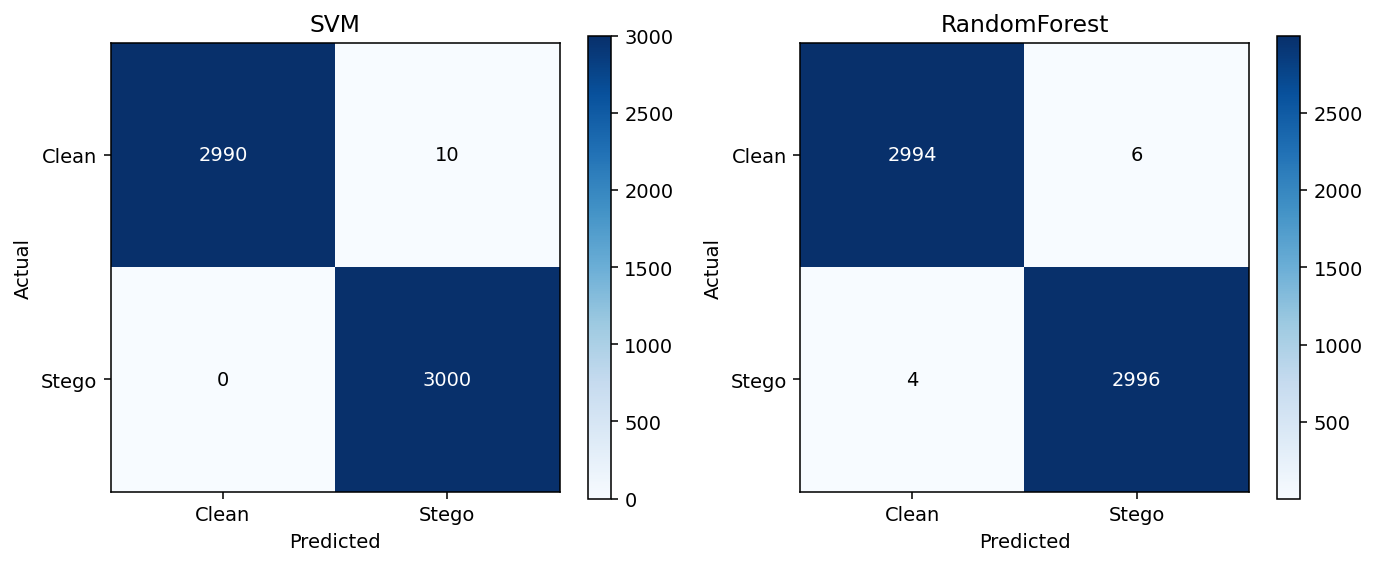
\includegraphics[width=0.82\linewidth]{results/confusion_matrices.png}
\caption{Matrices de confusion du test.}
\end{figure}

Interprétation : les métriques sont très hautes car la tâche est bien définie : détecter notre insertion LSB sur des images ALASKA préparées. Ce n'est pas une preuve que le modèle détecte toutes les méthodes de stéganographie modernes.

\section{Structure du projet}
Les fichiers importants sont les suivants :
\begin{longtable}{p{5cm}p{9cm}}
\toprule
Chemin & Rôle \\
\midrule
\texttt{app.py} & Interface Streamlit en français : détection, insertion, extraction, visualisations et métriques. \\
\texttt{detect.py} & Entrée ligne de commande pour tester une image ou une vidéo avec un modèle. \\
\texttt{run\_pipeline.py} & Script principal d'entraînement : préparation, features, modèles, seuils et résultats. \\
\texttt{src/lsb\_steganography.py} & Algorithmes d'insertion, extraction et calcul du PSNR. \\
\texttt{src/generate\_dataset.py} & Conversion ALASKA vers PNG propre et génération des images stego LSB. \\
\texttt{src/feature\_extractor.py} & Extraction des 218 caractéristiques. \\
\texttt{src/dataset\_pipeline.py} & Split par groupe et extraction parallèle des features. \\
\texttt{src/classifier.py} & Entraînement SVM/RF, calibration, évaluation, sauvegarde. \\
\texttt{models/} & Modèles entraînés : SVM, Random Forest et seuils. \\
\texttt{results/} & Métriques JSON et figures de validation. \\
\texttt{data/processed/} & Splits, labels et matrices de features. \\
\bottomrule
\end{longtable}

\section{Workflow complet d'entraînement}
\subsection{1. Préparation des paires}
Le script lit les images JPEG ALASKA. Pour chaque image, il crée une version propre PNG et une version stego PNG. Les deux images ont la même taille, le même format et la même origine.

Le message caché pendant l'entraînement est volontairement variable. Il peut être court, moyen ou long. Cela évite un modèle qui reconnaît seulement un seul type de payload.

\subsection{2. Split par groupe}
Le groupe est le nom de l'image source. La version propre et la version stego de la même image restent dans le même split. Cela évite une fuite de données : si le cover était dans train et le stego dans test, le modèle pourrait apprendre l'image au lieu d'apprendre la stéganographie.

\subsection{3. Extraction parallèle des features}
L'extraction des features est la partie lente. Le projet utilise \texttt{joblib.Parallel} avec plusieurs workers. Sur une machine correcte, il faut utiliser plusieurs processus, par exemple 15 workers, parce que traiter 40 000 images une par une en Python serait trop lent.

\subsection{4. Entraînement}
Le SVM et le Random Forest sont entraînés sur le split train. Quand l'option \texttt{--tune} est utilisée, le script cherche de meilleurs hyperparamètres. Après entraînement, les seuils sont ajustés sur la validation, pas sur le test.

\subsection{5. Test final}
Le test est utilisé une seule fois pour mesurer la performance finale. Les matrices de confusion et les courbes ROC sont sauvegardées dans \texttt{results/}.

\section{Trajet complet d'une image}
Cette section explique le projet comme une histoire complète, depuis l'image chargée jusqu'au verdict ou au texte extrait.

\subsection*{Cas 1 : l'utilisateur cache un texte}
\begin{enumerate}
  \item L'utilisateur charge une image.
  \item L'application convertit l'image en RGB et la redimensionne en 512 x 512.
  \item Le message est converti en octets UTF-8.
  \item Les octets sont convertis en bits.
  \item L'application construit un en-tête de 32 bits qui contient la taille du payload.
  \item Les bits sont écrits dans les LSB des valeurs RGB aplaties.
  \item L'image est sauvegardée en PNG pour protéger les LSB.
  \item L'application affiche l'image propre, l'image stego, la différence amplifiée, les plans LSB et le PSNR.
\end{enumerate}

Pourquoi cet ordre ? Parce qu'il sépare la préparation de l'image, la préparation du message, l'insertion binaire et la validation visuelle.

\subsection*{Cas 2 : l'utilisateur détecte une image}
\begin{enumerate}
  \item L'image est chargée en RGB.
  \item Elle est redimensionnée en 512 x 512 pour correspondre à l'entraînement.
  \item Les canaux RGB sont séparés.
  \item Les plans LSB sont extraits.
  \item Les features LSB, LBP, GLCM, histogrammes et moments sont calculées.
  \item Le vecteur de 218 valeurs est envoyé au SVM et au Random Forest.
  \item Chaque modèle renvoie une probabilité.
  \item La probabilité est comparée au seuil validé.
  \item L'application affiche le verdict et les mesures qui l'ont produit.
\end{enumerate}

Pourquoi afficher les étapes ? Parce que dans un cours de traitement d'images, le verdict seul n'est pas suffisant. Il faut montrer les transformations qui mènent au verdict.

\subsection*{Cas 3 : l'utilisateur extrait un texte}
\begin{enumerate}
  \item L'image PNG est chargée.
  \item Les LSB de toutes les valeurs RGB sont lus dans l'ordre.
  \item Les 32 premiers bits donnent la longueur du payload.
  \item Si la longueur est impossible, l'application arrête l'extraction.
  \item Sinon, elle lit le payload, reconstruit les octets et décode en UTF-8.
  \item Elle cherche le marqueur de fin.
  \item Elle affiche le texte seulement si le format est cohérent.
\end{enumerate}

Pourquoi cette prudence ? Parce qu'une image quelconque contient toujours des LSB. Sans validation, on pourrait afficher du texte faux.

\section{Décisions prises pendant la réalisation}
\begin{longtable}{p{4.1cm}p{5.0cm}p{5.0cm}}
\toprule
Ce que nous avons fait & Pourquoi nous l'avons fait & Ce que cela évite \\
\midrule
Nous sauvegardons les sorties en PNG & Le PNG est sans perte et conserve les LSB. & La recompression JPEG qui peut détruire le message caché. \\
Nous avons choisi des features interprétables & Elles correspondent à des notions de traitement d'images vues en cours. & Une boîte noire qui donne un verdict sans expliquer les transformations. \\
Nous utilisons SVM et Random Forest & Les deux modèles donnent deux lectures différentes des mêmes features. & Dépendre d'un seul modèle sans comparaison. \\
Nous avons fait un split par groupe & Une image source et sa version stego restent dans le même ensemble. & Une fuite de données qui gonfle artificiellement les scores. \\
Nous validons les seuils & Le score continu devient un verdict avec un seuil mesuré sur validation. & Utiliser 0,5 par habitude même quand ce n'est pas optimal. \\
Nous affichons les étapes visuelles & L'utilisateur voit les canaux, les plans LSB et les mesures réelles. & Une application qui cache le traitement et montre seulement une conclusion. \\
\bottomrule
\end{longtable}

\section{Construction des outils du projet}
\subsection*{Outil 1 : insertion LSB}
Nous avons construit l'outil d'insertion pour transformer un texte en modification mesurable de l'image. Le texte est d'abord encodé en UTF-8, puis transformé en bits. Nous ajoutons un en-tête de 32 bits pour enregistrer la longueur du message, puis un marqueur de fin pour vérifier que l'extraction est cohérente.

Ensuite, nous parcourons les valeurs RGB comme un long tableau. Pour chaque bit du message, nous remplaçons le LSB de la valeur RGB correspondante. Si le bit était déjà correct, la valeur ne change pas. Sinon, elle change seulement de 1. C'est pour cela que l'image reste presque identique visuellement.

\subsection*{Outil 2 : extraction LSB}
Nous avons construit l'extracteur comme l'inverse exact de l'insertion. Il lit les LSB dans le même ordre. Les 32 premiers bits donnent la taille à lire. Après cela, l'outil lit le payload, reconstruit les octets et décode le texte en UTF-8.

Nous avons ajouté des validations parce qu'une image quelconque possède toujours des LSB. Sans vérifier la taille et le marqueur de fin, l'application pourrait afficher du texte faux. Donc l'outil n'affiche le message que si le format correspond à notre protocole.

\subsection*{Outil 3 : visualisation de traitement d'images}
Nous avons ajouté des visualisations pour que l'application montre le traitement, pas seulement le résultat. Pour chaque image, elle affiche les canaux rouge, vert et bleu, les plans LSB, les histogrammes, la différence amplifiée et une carte LBP.

Ces images intermédiaires sont calculées à partir de l'image courante. Elles ne sont pas un guide statique. Elles montrent vraiment comment l'image chargée est transformée en données exploitables.

\subsection*{Outil 4 : extraction des caractéristiques}
Nous avons construit un extracteur de features pour résumer l'image en 218 valeurs. Cela permet de passer d'une image 512 x 512 x 3, donc 786 432 valeurs RGB, à un vecteur compact. Ce vecteur garde les informations utiles pour notre problème : structure des LSB, texture, distribution des couleurs et moments statistiques.

Cette étape est le coeur image-processing du projet. Les modèles ne regardent pas directement les pixels bruts ; ils utilisent les mesures que nous avons calculées.

\subsection*{Outil 5 : entraînement et détection}
Nous avons construit le pipeline d'entraînement pour générer les paires clean/stego, extraire les features en parallèle, entraîner les modèles, calibrer les seuils, puis sauvegarder les résultats. L'application charge ensuite les modèles sauvegardés et applique exactement le même extracteur de features sur l'image de l'utilisateur.

Cette cohérence est importante : l'image testée doit être traitée comme les images d'entraînement. Sinon, les probabilités affichées ne seraient pas fiables.

\section{Ce que nous avons corrigé pendant la réalisation}
Au début, le risque principal était d'obtenir de bons scores pour une mauvaise raison. Nous avons donc modifié le pipeline pour que les images propres et stego soient toutes les deux en PNG. Cela empêche le modèle d'apprendre simplement le format du fichier.

Nous avons aussi changé le split des données. Les paires venant de la même image source restent ensemble. Cela évite que le modèle voie une version d'une image pendant l'entraînement et l'autre pendant le test.

Enfin, nous avons amélioré l'application pour qu'elle affiche des étapes réelles : pas seulement des phrases comme \og l'image est redimensionnée \fg{}, mais les images intermédiaires, les ratios, les tailles, les plans de bits et les probabilités calculées.

\section{Interpréter les métriques}
La matrice de confusion a quatre cases :
\begin{itemize}
  \item vrai propre : image propre correctement classée propre ;
  \item faux positif : image propre classée stego ;
  \item faux négatif : image stego classée propre ;
  \item vrai stego : image stego correctement classée stego.
\end{itemize}

Pour le SVM, la matrice est \texttt{[[2990, 10], [0, 3000]]}. Cela veut dire 10 faux positifs et 0 faux négatif sur le test. Pour le Random Forest, la matrice est \texttt{[[2994, 6], [4, 2996]]}. Cela veut dire 6 faux positifs et 4 faux négatifs.

Le recall mesure la capacité à trouver les images stego. La précision mesure la fiabilité quand le modèle dit \og stego \fg{}. Le F1 combine les deux. L'AUC mesure la qualité du classement quand on fait varier le seuil.

\begin{figure}[h]
\centering
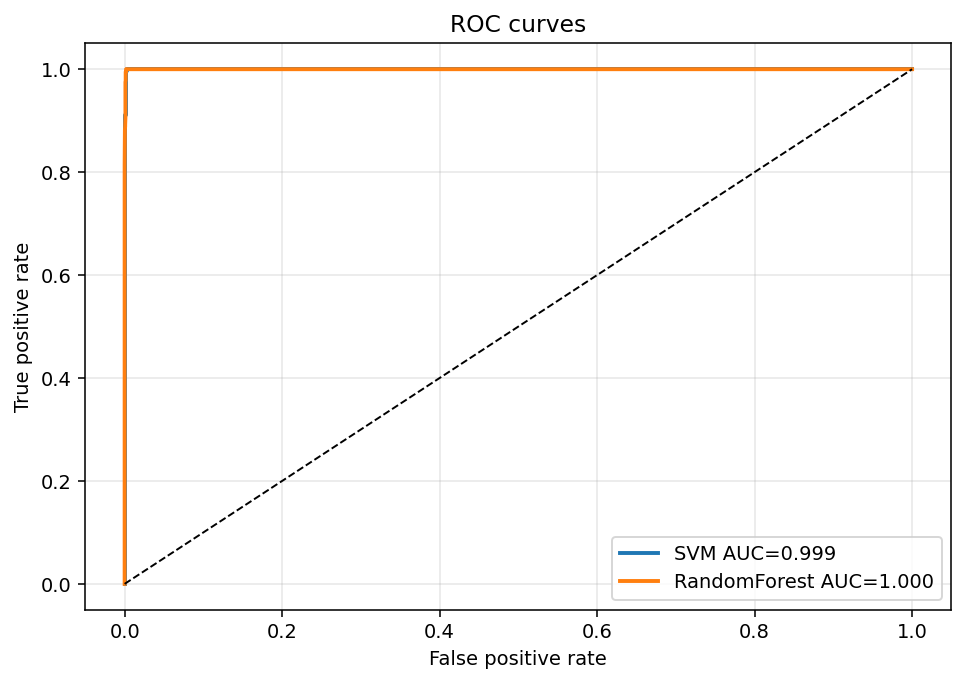
\includegraphics[width=0.78\linewidth]{results/roc_curves.png}
\caption{Courbes ROC sauvegardées après l'entraînement.}
\end{figure}

\begin{figure}[h]
\centering
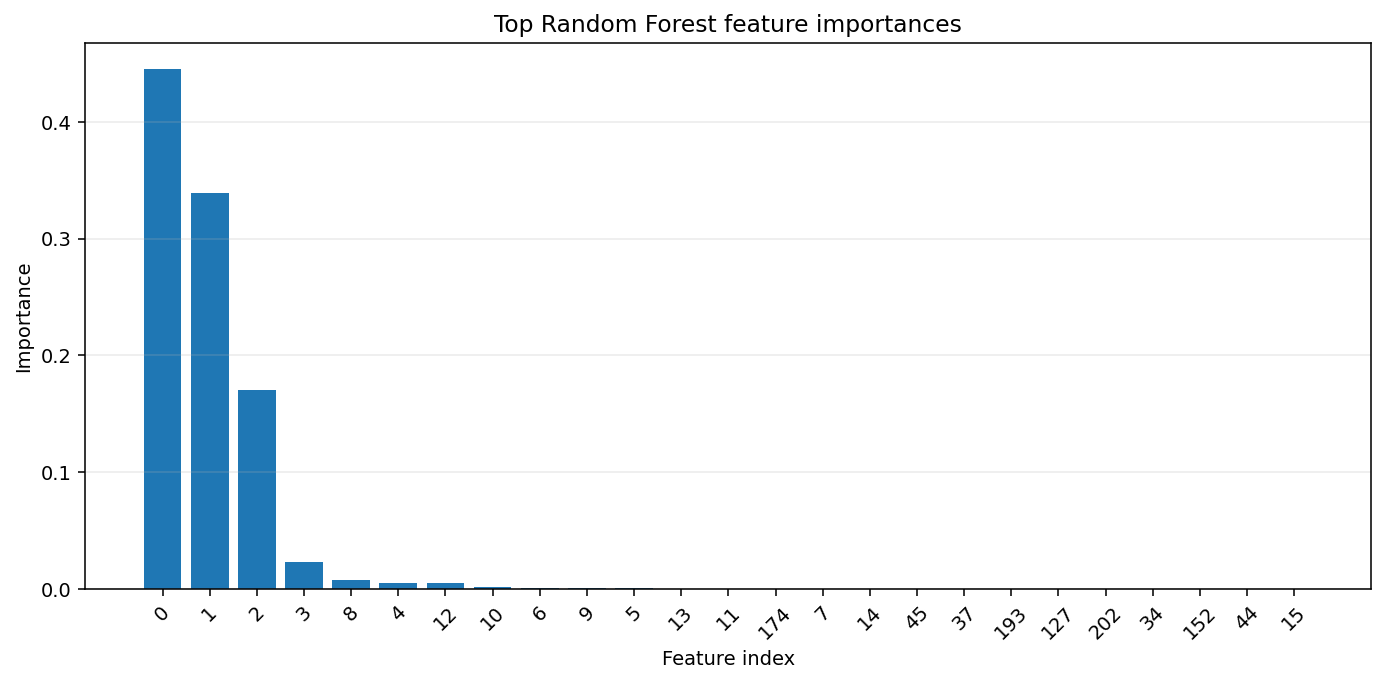
\includegraphics[width=0.78\linewidth]{results/feature_importance.png}
\caption{Importance des features pour le Random Forest.}
\end{figure}

\section{Pourquoi les scores peuvent sembler très hauts}
Des scores proches de 99,8 \% peuvent sembler suspects. Ils sont acceptables ici seulement si on explique la tâche exacte :
\begin{itemize}
  \item les images stego sont produites par notre propre méthode LSB ;
  \item le format propre/stego est contrôlé et identique ;
  \item le modèle voit des indices très directs, comme l'en-tête LSB de 32 bits ;
  \item le test est séparé par groupe, donc il n'y a pas de paire train/test issue de la même image.
\end{itemize}

Ces scores seraient anormaux si on prétendait détecter toutes les stéganographies JPEG. Mais pour notre problème contrôlé, ils sont cohérents.

\section{Contrôles et smoke tests}
Avant une démonstration, il faut vérifier :
\begin{enumerate}
  \item que \texttt{models/svm\_model.pkl}, \texttt{models/rf\_model.pkl} et \texttt{models/thresholds.json} existent ;
  \item que \texttt{results/metrics.json} correspond au dernier entraînement ;
  \item qu'une image propre ALASKA obtient une probabilité basse ;
  \item qu'une image produite par l'onglet insertion obtient une probabilité haute ;
  \item que l'extraction retrouve exactement le message.
\end{enumerate}

Un test minimal consiste à cacher un court texte dans une image, lancer la détection sur l'image propre puis sur l'image stego, et extraire le message. Si ces trois opérations fonctionnent, le coeur du projet est prêt.

\section{Détail de l'interface}
\subsection{Onglet Détecter}
L'utilisateur charge une image. L'application affiche le verdict, puis les étapes visuelles sous l'image et sous le verdict. Les données affichées sont recalculées pour l'image courante : ratios LSB, en-tête, features, probabilités et seuils.

\subsection{Onglet Cacher du texte}
L'utilisateur peut choisir de cacher un texte ou de ne rien cacher. L'option sans texte sert de contrôle : elle produit une image comparable pour tester si le modèle invente un verdict stego. Quand un texte est caché, l'application montre la différence amplifiée, le PSNR et les plans LSB après insertion.

\subsection{Onglet Extraire}
L'utilisateur charge un PNG. L'application lit l'en-tête et le payload. Elle affiche les plans LSB lus, la longueur annoncée, la validité et le texte extrait.

\section{Erreurs courantes et solutions}
\begin{longtable}{p{5cm}p{9cm}}
\toprule
Problème & Solution \\
\midrule
Le message ne s'extrait pas & Vérifier que l'image est bien le PNG stego, pas une capture ou un JPEG recompressé. \\
Le modèle donne un verdict inattendu & Comparer SVM et RF, regarder les seuils et tester avec une image produite par l'application. \\
L'entraînement est lent & Augmenter \texttt{--workers}, garder les features en cache quand on teste seulement les modèles. \\
Les accents s'affichent mal dans PowerShell & Le fichier peut être correct en UTF-8 même si la console affiche mal. Vérifier avec Python ou ouvrir dans l'éditeur. \\
Le PPTX ne s'écrase pas & Fermer PowerPoint ou Google Drive Sync, ou générer un nouveau fichier corrigé. \\
\bottomrule
\end{longtable}

\section{Synthèse image-processing du projet}
La partie importante du projet est le traitement d'images :
\begin{itemize}
  \item on manipule directement les pixels et les bits ;
  \item on visualise les canaux et les plans LSB ;
  \item on extrait des caractéristiques classiques de texture ;
  \item les modèles ne remplacent pas l'explication visuelle, ils utilisent les mesures produites par le traitement d'images.
\end{itemize}

Cette synthèse montre ce que nous avons vraiment construit : un système qui part des pixels, extrait des représentations visuelles et statistiques, puis utilise ces mesures pour cacher, lire ou détecter un message.

\section{Commandes importantes}
Installation :
\begin{lstlisting}
python -m pip install -r requirements.txt
\end{lstlisting}

Entraînement complet sur les 20 000 images cover :
\begin{lstlisting}
python run_pipeline.py --workers 15 --tune --force-stego --force-features
\end{lstlisting}

Entraînement rapide de test :
\begin{lstlisting}
python run_pipeline.py --smoke --workers 8
\end{lstlisting}

Détection en ligne de commande :
\begin{lstlisting}
python detect.py --image image.png --model rf --json
python detect.py --image image.png --model svm --json
\end{lstlisting}

Application :
\begin{lstlisting}
streamlit run app.py
\end{lstlisting}

\section{Workflow de démonstration conseillé}
\begin{enumerate}
  \item Ouvrir l'application Streamlit.
  \item Aller dans \textbf{Cacher du texte}.
  \item Charger une image, saisir un petit message, puis créer le PNG stego.
  \item Montrer l'image propre, l'image stego, la différence amplifiée et les plans LSB.
  \item Aller dans \textbf{Détecter}.
  \item Tester d'abord l'image propre, puis le PNG stego.
  \item Lire les probabilités SVM/RF et expliquer les seuils.
  \item Aller dans \textbf{Extraire le texte}.
  \item Charger le PNG stego et montrer la lecture de l'en-tête puis du payload.
\end{enumerate}

\section{Limites du système réalisé}
\begin{itemize}
  \item Le modèle est spécialisé dans le LSB généré par notre application.
  \item Les méthodes comme JMiPOD, J-UNIWARD et UERD demanderaient des données stego correspondantes.
  \item Les petits messages peuvent être plus difficiles à détecter si on retire l'indice d'en-tête propre à l'application.
  \item Les images JPEG recompressées peuvent détruire le message LSB.
  \item Les excellents scores ne doivent pas être présentés comme une stéganalyse universelle.
\end{itemize}

\section{Ce qu'il faut retenir}
Le projet relie directement le cours de traitement d'images à une application pratique. On part d'une matrice RGB, on manipule les bits, on visualise les canaux et les plans LSB, on extrait des caractéristiques de texture et de statistiques, puis on utilise un classificateur pour prendre une décision.

\end{document}
